\documentclass[landscape]{article}

\usepackage[top=.5in, bottom=1in, left=1in, right=1in]{geometry}

\usepackage{graphicx}
\usepackage{float}
\usepackage{hyperref}


\author{Brian Kennedy, Pete Koehn, Theodore Lindsey}
\title{EECS 448 \\ Report 2: Design Philosophy and Diagrams}

\begin{document}
\maketitle

\vfill

\tableofcontents

\newpage

\

\newpage

\section{Agile Methodology of Choice: Extreme Programming (XP)}

The Agile methodologies are built around several principles, including customer involvement, incremental product delivery, and simplicity. Some of the important aspects of XP include the creation of user story cards, a task-based development cycle, and the development of testing methods before coding begins. During the XP development cycle, several strategies may be implemented to deal with obstacles or challenges that might be encountered. These include refactoring, spike programming, and pair programming. We do not have initial plans to implement any of these strategies, but they remain available to us if necessary.

For this project, we will develop user story cards. These user story cards will be broken down into their individual tasks, and will subsequently be assigned to individual team members. A broad picture of this process was provided in the form of a Gantt chart in Part 1 of the project. Once the user stories are developed and the tasks have been delineated, tests for each task will be developed. It is important the tests be developed before coding begins.

\section{User Stories}
\subsection{User Story, Case 1: Recipe Import}

A user wishes to upload a properly formatted recipe stored on their local machine into the application's recipe database. The user launches the application and selects `Import a Recipe' from the application window. The user is prompted to enter the folder location where the recipe is stored, as well as the name of the recipe file. If a specified file is found in the given directory, the program will import the recipe, and the interaction is complete.


\subsection{Tests, Case 1}

The user will be required to input a valid file folder location. The user is also required to input a valid and accessible filename. If no file can be found in the given directory that contains the given filename, the user will be asked to re-input both the file folder location and the filename.

\subsection{User Story, Case 2: Add Recipe}

A user wishes to add a recipe to the application's recipe database by entering the recipe information into the application window directly. The user will launch the application and select `Add a Recipe'. The user will then be prompted to enter information for the various recipe fields (name, number of servings, bake/cook time, ingredients, etc.). Once the user has added information for each field, the application will add the new recipe to the database, and the interaction is complete.

\subsection{Tests, Case 2}

As all user input in this case is taken in the form of a string, only a set of very simple tests will be implemented. For example, if the user enters a string of letters for the number of servings, they will be prompted to provide valid input, i.e., an integer. Similar tests can be implemented for bake/cook time.

\subsection{User Story, Case 3: Modify Recipe}

A user wishes to modify an existing recipe in the application's recipe database. The user will launch the application and select `Modify a Recipe' from the application window. The user will be prompted to enter the name of the recipe. The requested recipe's information will be displayed for the user to review, and they will be prompted to input the name of the field or fields they wish to modify. For each field to be modified, the user will be prompted to input new information that will replace the existing information. When the user is satisfied, they will save the recipe, and the interaction is complete.

\subsection{Tests, Case 3}

Like the tests for Case 2, only simple tests can be implemented on the user input in Case 3.

\subsection{User Story, Case 4: PDF Compilation}

A user wishes to generate a PDF of all of the recipes in the application's recipe database. The user will launch the application and select `Generate PDF'.  The user will be prompted to select which Tables of Contents they would like included in the PDF. The recipes will be indexed by a series of Tables of Contents that include: name, style, ethnicity, etc. Once the user has selected the desired Tables of Contents, the PDF will be generated for the user. The PDF can be found in the application's source folder.

\subsection{Tests, Case 4}

No tests are to be implemented in this case.

\subsection{User Story, Case 5*: Recipe Website Fetch}

A user wishes to load a recipe into the application’s recipe database from a website, e.g., \href{http://allrecipes.com/}{AllRecipes.com}. The user will launch the application and select `Load Recipe from Web'. The user will be prompted to enter the exact URL of the webpage containing the recipe. This will be most efficiently done by copying and pasting the address from the browser. Once the user has inputted an acceptable URL, the application will automatically convert and import the given recipe.

*This functionality has the lowest priority, but we hope to incorporate it as time allows.

\subsection{Tests, Case 5}

As this task requires complex interfacing with external websites, this feature will be limited to work with only a select number of websites. Error handling will be quite general, but the user will be informed if the given URL does not provide a recipe that the application can process.


\section{Version Control}

A Github repository (\href{https://github.com/RagingRoosevelt/eecs448fp}{github.com/RagingRoosevelt/eecs448fp}) has been and will be used to store different pieces of the project for viewing and editing by team members. Team members will upload their contributions to the project and make comments telling the other team members what changes they have made.  Given the separation of tasks, it has not been necessary to branch the repository and everyone has successfully worked with the main branch.

\newpage

\section{Diagrams}

\begin{figure}[H]
\begin{centering}
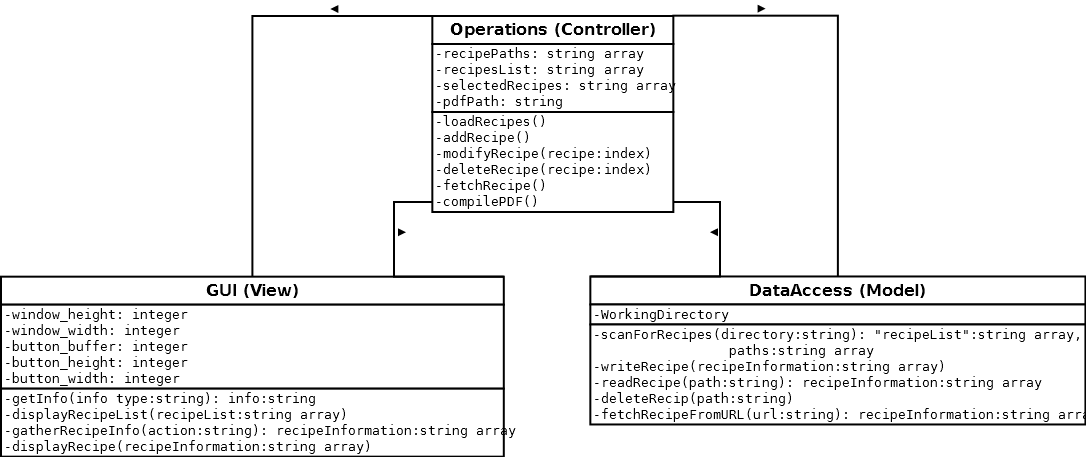
\includegraphics[width=\textwidth]{Diagram-Class.png}
\caption{Class Diagram}
\end{centering}
\end{figure}


\begin{figure}[H]
\begin{centering}
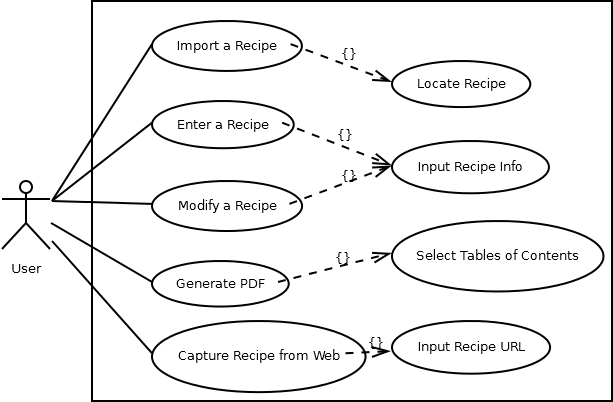
\includegraphics[width=0.75\textwidth]{Diagram-UseCase.png}
\caption{Use Case Diagram}
\end{centering}
\end{figure}

\begin{figure}[H]
\begin{centering}
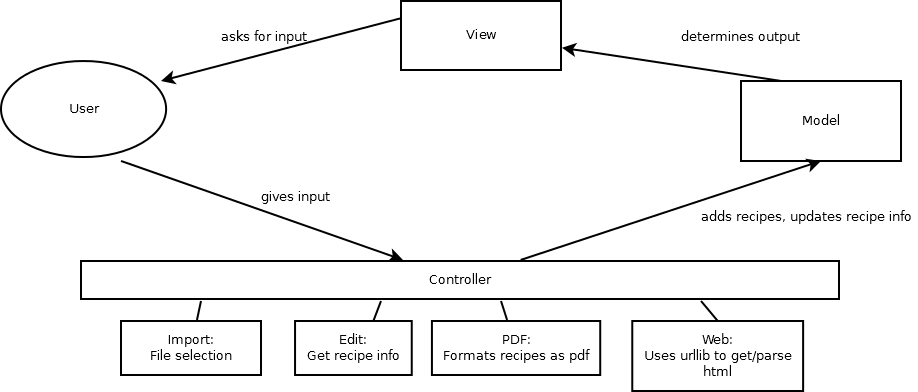
\includegraphics[width=0.75\textwidth]{Diagram-SystemArchitecture.png}
\caption{System Architecture Diagram}
\end{centering}
\end{figure}

\begin{figure}[H]
\begin{centering}
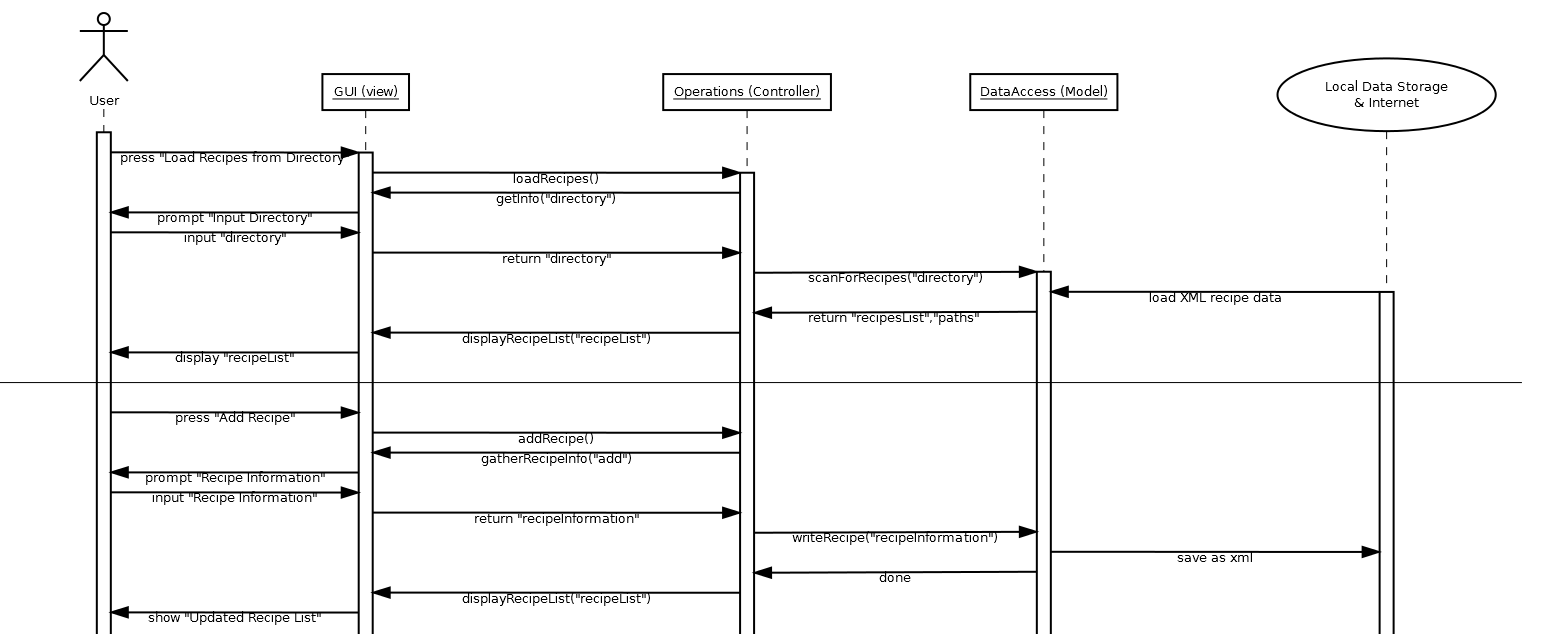
\includegraphics[width=\textwidth]{Diagram-SequenceA.png}
\caption{Sequence Diagram (pt 1)}
\end{centering}
\end{figure}

\begin{figure}[H]
\begin{centering}
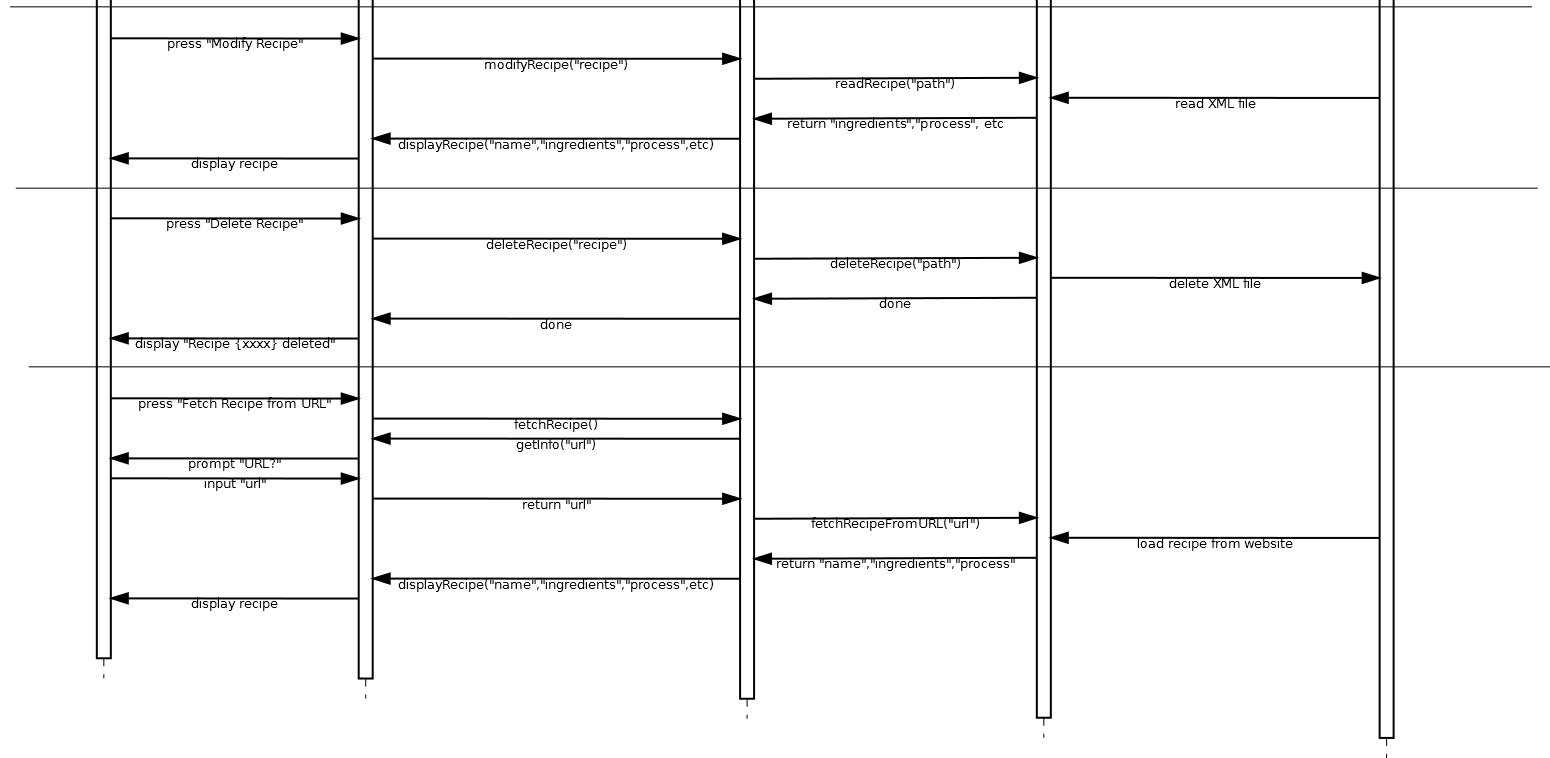
\includegraphics[width=\textwidth]{Diagram-SequenceB.png}
\caption{Sequence Diagram (pt 2)}
\end{centering}
\end{figure}



























\end{document}